% Modified based on Xiaoming Sun's template and https://www.overleaf.com/latex/templates/cs6780-assignment-template/hgjyygbykvrf

\documentclass[a4 paper,12pt]{article}
\usepackage[inner=2.2cm,outer=2.2cm,top=2.5cm,bottom=2.5cm]{geometry}
\usepackage{setspace}
\usepackage[rgb]{xcolor}
\usepackage{verbatim}
\usepackage{subcaption}
\usepackage{fancyhdr}
\usepackage[colorlinks=true, urlcolor=blue, linkcolor=blue, citecolor=blue]{hyperref}
\usepackage{booktabs}
\usepackage{amsmath,amsfonts,amsthm,amssymb}
\usepackage{setspace}
\usepackage{fancyhdr}
\usepackage{lastpage}
\usepackage{extramarks}
\usepackage{indentfirst}
\usepackage{chngpage}
\usepackage{soul,color}
\usepackage{bm}
\usepackage{graphicx,float,wrapfig}
\usepackage{tikz}
\setlength{\parindent}{2em}
\usetikzlibrary{positioning}
\usetikzlibrary{arrows,graphs}
\newcommand{\homework}[3]{
   \pagestyle{myheadings}
   \thispagestyle{plain}
   \newpage
   \setcounter{page}{1}
   \noindent
   \begin{center}
   \framebox{
        \vbox{\vspace{2mm}
        \hbox to 6.28in { {\bf Causal and Statistical Inference \hfill} {\hfill {\rm #2} {\rm #3}} }
        \vspace{4mm}
        \hbox to 6.28in { {\Large \hfill #1  \hfill} }
        \vspace{3mm}}
   }
   \end{center}
   \vspace*{4mm}
}
\newcommand\numberthis{\addtocounter{equation}{1}\tag{\theequation}}

% Custom defined operators
\DeclareMathOperator{\Do}{do}

\begin{document}
\homework{Poster Report: RDD}{Kai Su,}{Qihang Chen}

\section{Analyzing Baysian Network}
\subsection{Introduction to RDD}
When the running variable $X$ takes value at different side of a threshold value $t$, there will be a treatment(marked $w=1$) having an effect on the output $Y$ on one side of $X=t$ and no treatment(marked $w=0$) on the other side. Our goal is to measure the average effect $\tau$ solely caused by the treatment. That is, $\tau=E[Y|\Do(W)=1]-E[Y|\Do(W)=0]$.

Such effect appears as a sudden increase or decrease of $y$ in the neighborhood of $X=t$(See Fig.\ref{fig:rddintro}). Therefore, $\tau$ is traditionally estimated using the see effect of $W$. Formally put,

\begin{equation}
   \hat\tau=\lim_{x\to t^+}E[Y|X=x]-\lim_{x\to t^-}E[Y|X=x].\label{eqn:est_lim}
\end{equation}

For simplicity, denote 
\begin{align}
   E[Y|X=t_+]=\lim_{x\to t^+}E[Y|X=x],\\
   E[Y|X=t_-]=\lim_{x\to t^-}E[Y|X=x].
\end{align}

However, we are lack of data near the threshold in most cases, difficult for us to calculate these values on the threshold directly. Thus we need some regression to infer the relation between $X$ and $Y$ so as to predict $E[Y|X=t_+]$ and $E[Y|X=t_-]$.

A common practice is to apply linear regression on both sides. The data near the threshold is more valuable, thus we can set a bandwidth $b$, which is the largest distance where data are taken into account; and a kernel $k$, which assigns weights to data.

\begin{figure}[h]
	\centering
   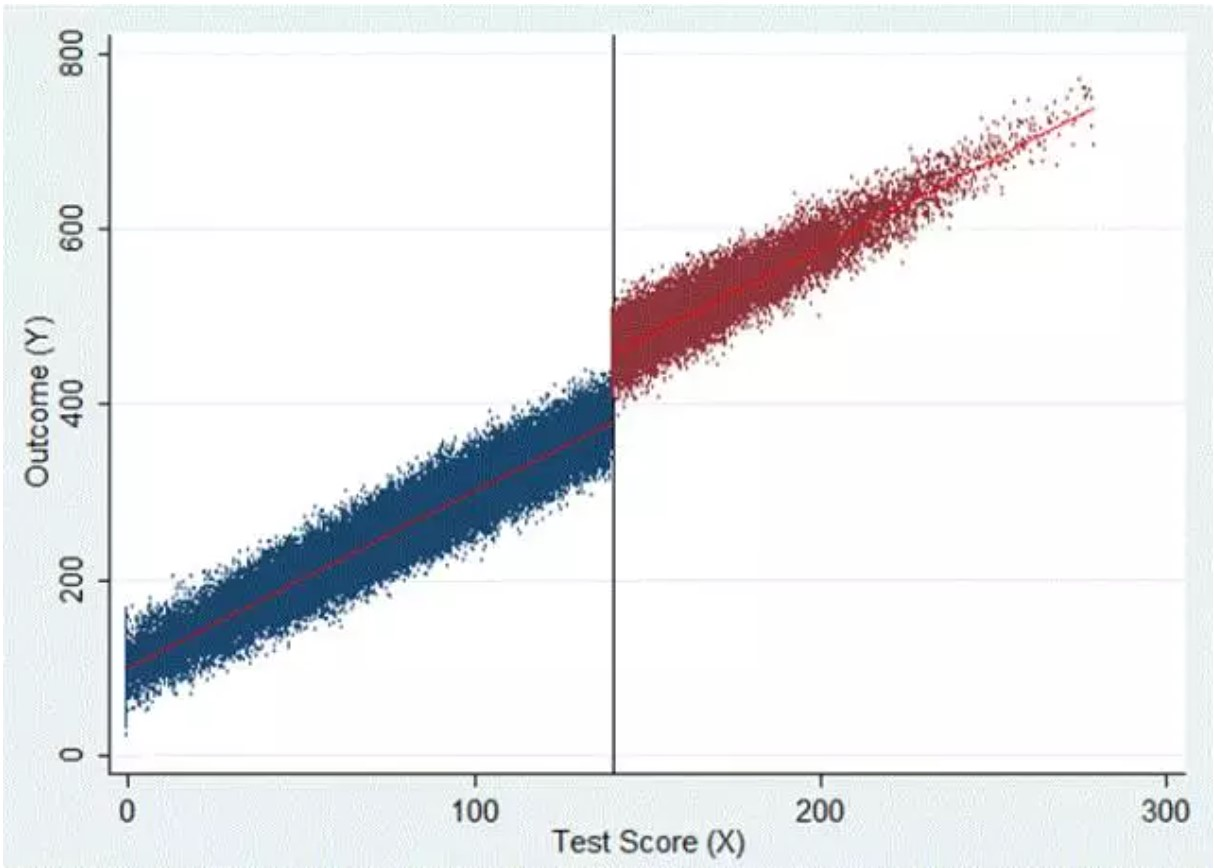
\includegraphics[scale=1]{RDDintro.jpg}
   \caption{An example of dataset in RDD}
   \label{fig:rddintro}
\end{figure}

\subsection{Baysian Network}
Basically, running variable $X$ will decide $W$ and affect $Y$; $W$ will have effect on $Y$, as in Fig.\ref{fig:basic_rd_bns}.

\begin{figure}[h]
	\centering
   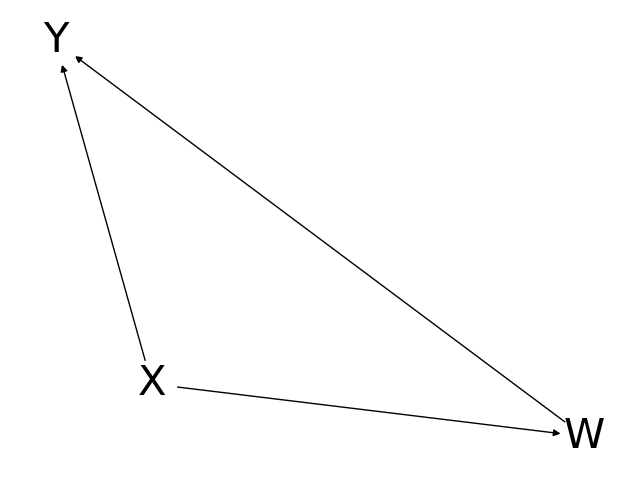
\includegraphics[scale=0.5]{Figure_1.png}
   \caption{The basic BN for RDD}
   \label{fig:basic_rd_bns}
   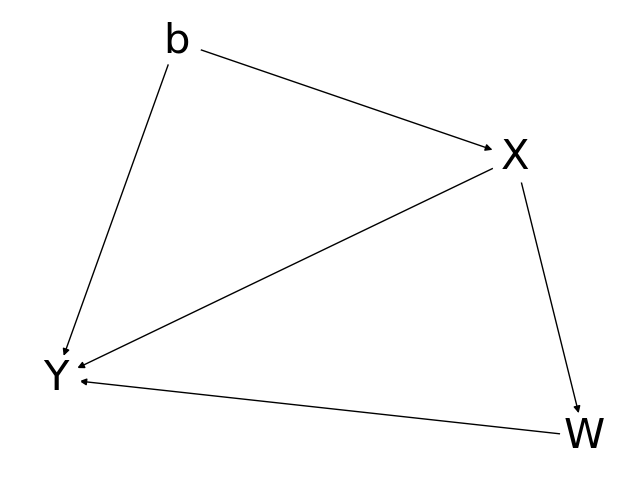
\includegraphics[scale=0.5]{Figure_2.png}
   \caption{BN with bandwidth}
   \label{fig:bn_with_bdw}
\end{figure}

\subsection*{bandwidth}
When the bandwidth is sufficiently small,
\begin{align}
   P[Y|W=0]\approx P[Y|X=t_-],\\
   P[Y|W=1]\approx P[Y|X=t_+].
\end{align}

Then
\begin{align}
   \tau=E[Y|\Do(W)=1]-E[Y|\Do(w)=0]\approx E[Y|X=t_+]-E[Y|X=t_-]=\hat\tau,
\end{align}

proving that the traditional estimation in Eqn.(\ref{eqn:est_lim}) is unbiased.

In contrast, if the bandwidth $b$ is non-negligible, this selection of data specified by $b$ will cause a backdoor path between $X$ and $Y$. (See Fig.\ref{fig:bn_with_bdw}) Then the see effect observed by regression between $X$ and $Y$ is not the true causal effect, leading to a bias. To eliminate this bias, we need to adjust the way of sampling by changing the kernel.

\subsection*{covariates}
Sometimes there are not only running variables $X$ and $Y$, but also many other variables $Z$, called covariates, may have effect on $Y$. If they are independent with $X$, the regression still works. However in some cases, $Z$ will affect both $X$ and $Y$, creating a backdoor path between $X$ and $Y$. (See Fig.\ref{bn_with_covar})

In order to eliminate this bias, we need to find a bandwidth, to make sure among the included samples, $Z$ is independent with $X$.

\begin{figure}[h]
	\centering
	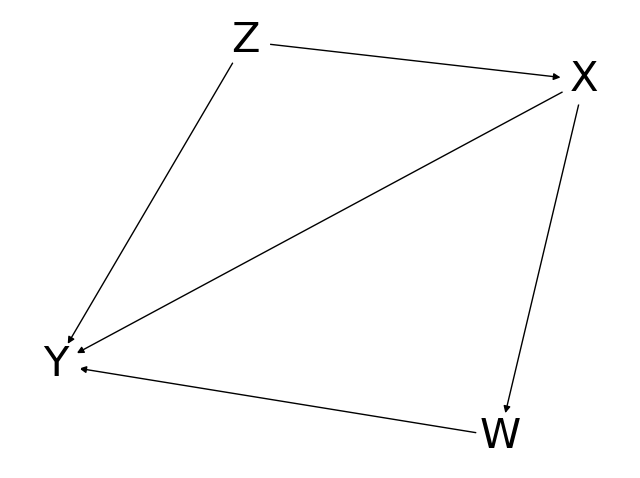
\includegraphics[scale=0.5]{Figure_3.png}
   \caption{BN with covariates}
   \label{bn_with_covar}
	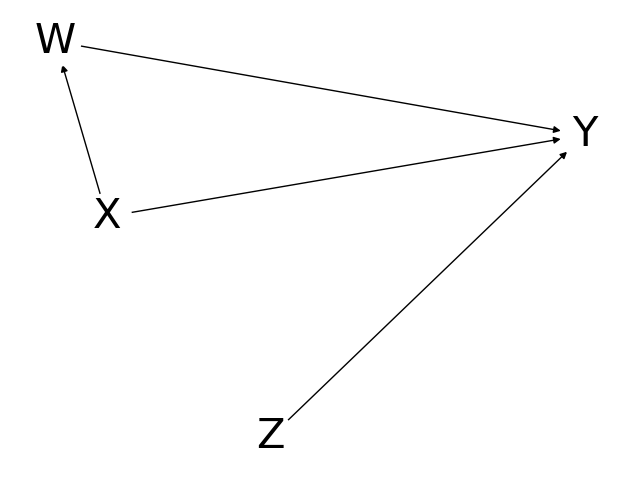
\includegraphics[scale=0.5]{Figure_4.png}
\end{figure}

\section{Experiment and Discussion}

\subsection{Using kernel to elimimate bias caused by bandwidth}

In this section we do not consider covariates. We generate data by different $X-Y$ relation and different distribution of samples. 
%这里我好像有点忘了当时编号和数据的关系了,你帮忙解释一下每组代表什么样的分布

We randomly generated 500 groups of data and 200 different types of kernels. For each kernel, we calculate the difference of $Y$ at threshold compared with $Y(t)$ by True $X-Y$ relation in those 500 groups of data, getting the average to show the performance of the kernel. Thus we get the best kernel for different bandwidth.
%你先介绍一下典型结果

\subsection{ Differences after adding covariates}
After adding covariates, there will be another backdoor path caused by $Z$, and the perfomance of different kernels may become different.


\section{Other Attempts}
\subsection*{A better way to find best bandwidth}

In some articles, cross validation method is used for selecting a optimal bandwidth. However this has not always accurate because samples near threshold may not have similar distribution and $X-Y$ relation.

When bandwidth is large, the $X-Y$ relation's nonlinearity may cause bias if using linear regression. When bandwidth is small, there may be too few samples, leading to a high variation.

We have these ways to quantify the expected error for different bandwidth caused by two aspects above:

(1) Use bandwidth $b$, suppose the linear regression has the result $Y=a(X-t)+b$, we use a formula to calculate the standard derivation of $b$ two represent the expected error caused by lack of data near threshold.

(2) First use a quadratic hypothesis function on regression to find out a curve showing approximate quadratic relationship between $X-Y$(do not use bandwitdh $b$). Then project all the samples onto the curve, use linear regression with bandwidth $b$ and find the difference of value between the two ways of regression on the threshold. 

Then we find a bandwidth who has least sum of those two kind of errors, just the optimal bandwidth we need.

\begin{figure}[h]
	\centering
	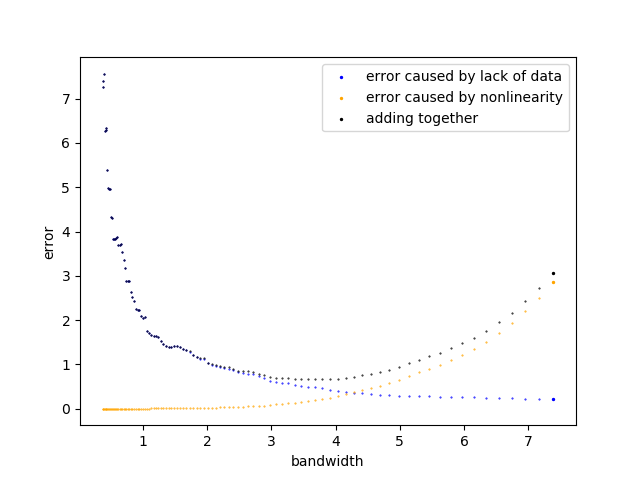
\includegraphics[scale=1]{Figure_5.png}
\end{figure}




\end{document} 
